\documentclass[10pt]{article}
% Submission build (anonymous). Camera-ready: \usepackage[accepted]{tmlr}.
% Preprint: \usepackage[preprint]{tmlr}.
\usepackage{tmlr}

\usepackage{amsmath,amssymb}
\usepackage{booktabs}
\usepackage{graphicx}
\usepackage{hyperref}
\usepackage{url}
\hypersetup{colorlinks=true,linkcolor=blue,citecolor=blue,urlcolor=blue}

\title{Quantization Sensitivity Follows the Consuming Operator}

\author{\name Anonymous authors \\
      \addr Paper under double-blind review}

\def\month{MM}
\def\year{YYYY}
\def\openreview{\url{https://openreview.net/forum?id=XXXX}}

\newcommand{\KL}{\mathrm{KL}}

\begin{document}

\maketitle

\begin{abstract}
Weight quantization is often guided by a ranking of a model's components built from
statistics of their weights. We test such a ranking for the four attention projections.
With the same per-output-channel quantizer at the same bit width, the relative Frobenius
errors of the four projections are similar, yet at 4 bits perturbing the value and output
projections moves the next-token distribution 2.4 to 3.8 times more than perturbing the query
and key projections, on four models. A recently reported ranking, built from weight statistics
under llama.cpp schemes, puts query and key first. We do not refute that ranking under its own
protocol. A factorial on two models shows where the two orderings part: the shipped llama.cpp
presets give query and key fewer bits, which raises their weight-statistic distortion, and at
equal bits under the same scheme the weight statistics tie while the output still moves 4 to 17
times more under value and output. Below 4 bits no stable ordering remains. On Llama-3.2-3B a
3-bit key projection fails, and the damage rises with the rotary wavelength of the key rows. At a
matched budget of 3.625 bits per key weight on held-out text, protecting the longest-wavelength
eighth of the rows removes 89\% of the damage, against 6\% to 37\% for a random eighth, but the
eighth with the largest weight error removes 96\%, so wavelength is not the best criterion. For
top-$k$ routers, the ratio of the spread of the logit error to the routing margin separates a
router that mostly keeps its routes at 4 bits from one that loses nearly all of them. For a
state-space model, a 3-bit grid on the logarithm of the decay rate keeps perplexity near the
baseline, while two linear grids collapse it, on two checkpoints.
\end{abstract}

\section{Introduction}\label{sec:intro}

A quantized tensor is usually accepted by one of three checks. Its reconstruction error is
small. The model's accuracy or perplexity stays close to the baseline. Or the component it
belongs to ranks low in a sensitivity order built from weight statistics. All three checks
look at the tensor itself or at an aggregate over the whole model. None of them looks at the
operation that reads the tensor.

The cost of that omission showed up in an earlier study of key-value cache compression
\citep{anon2026overview}. A per-vector quantizer applied to cached attention keys
reconstructed them better than a 3-bit per-channel quantizer, and its perplexity was 675
times higher. The per-vector quantizer stores each key's norm and quantizes its direction at
4 bits. Normalization alone does not discard the per-channel structure that the attention
score reads, and more directional bits could recover it, so the failure is a misallocation at
a fixed budget. Per-channel key quantization was already known to work
\citep{liu2024kivi,hooper2024kvquant}. The lesson was about acceptance. A reconstruction check
passed a quantizer that the consumer of the tensor could not use.

This paper asks the same question of weight quantization, where precision is often allocated
by a ranking of components. \citet{rababah2026illusion} rank the attention projections by
statistics and divergences of their weights under the quantization schemes of llama.cpp
\citep{gerganov2023llamacpp}, and find the query and key projections the most sensitive.
Section~\ref{sec:proj} gives every projection the same per-output-channel quantizer at the
same bit width and reads sensitivity at the model's output. The relative Frobenius errors of
the four projections are then similar, and the value and output projections move the output
more. Our protocol differs from theirs in bit allocation, quantization scheme and sensitivity
metric at once. Section~\ref{sec:proj:factorial} therefore crosses those factors on two models.
The reported ordering is reproduced by the weight statistics of the shipped presets, and it
follows the presets' bit allocation.

Below 4 bits the ordering breaks down. Section~\ref{sec:proj:below4} traces one failure, a
3-bit key projection on Llama-3.2-3B, to the key rows with the longest rotary wavelengths,
which SpQR had already found sensitive on another model \citep{dettmers2024spqr}. We localize
the damage by wavelength octile on two models and then test the protection against
budget-matched controls on held-out text. The long-wavelength rows are far better to protect
than random rows. They are not the best rows. An eighth chosen by weight error does better on
both models, and we report that against our own earlier reading.

Two further operators test the same claim outside attention. Section~\ref{sec:route} measures
top-$k$ routers on Mixtral-8x7B and OLMoE-1B-7B, and Section~\ref{sec:decay} measures the decay
of a linear recurrence on Mamba-790m. Section~\ref{sec:pullback} states the one definition the four studies share, the output
metric pulled back to the weights, and what would count against the paper's claim.
Section~\ref{sec:agree} describes the decision-level
measure we use throughout, which follows \citet{dutta2024accuracy} closely, and
Section~\ref{sec:trace} describes a tracer that assigns each tensor its consuming operator,
and measures how far it can be trusted.

We do not offer a better quantizer. We offer measurements of where each operator's fragility
lies, under declared protocols. All experiments use fake quantization on modest samples, and the
claims are relative and directional. Intervals, where given, come from resampling whole
sequences. Section~\ref{sec:limits} lists what is still missing, and the supplement holds a
notebook that rebuilds every reported number from the run records and a Lean file that checks
the paper's identities.

\section{Related work}\label{sec:related}

\paragraph{Beyond aggregate accuracy.} \citet{dutta2024accuracy} showed that compressed models
can match baseline accuracy while many answers flip, proposed the flip count as a distance
between models, and found that KL divergence tracks it. They also count changes from one wrong
answer to another, as AllFlips, and explain flips by small margins between the top answer
options. \citet{rababah2026illusion} introduced Correctness Agreement, the fraction of items
both models answer correctly, together with Cohen's kappa between the two models'
correctness. Our decision-level measure overlaps these closely. Its one addition is a
comparison with a reference perturbation, which we treat as descriptive.

\paragraph{Sensitivity in weight quantization.} Post-training methods such as GPTQ
\citep{frantar2023gptq}, LLM.int8() \citep{dettmers2022llmint8} and SmoothQuant
\citep{xiao2023smoothquant} treat outliers and error compensation. HAWQ
\citep{dong2019hawq,dong2020hawqv2} ranks layers by Hessian curvature to set mixed precision.
SpQR \citep{dettmers2024spqr} found, on LLaMA-65B, that query and key weights tied to
low-frequency rotary components \citep{su2024roformer} are more sensitive than those tied to
high frequencies. Section~\ref{sec:proj:below4} builds on that observation with a localization
by wavelength octile, a quantified intervention and a replication.

\paragraph{Key-value caches.} KIVI \citep{liu2024kivi} and KVQuant \citep{hooper2024kvquant}
quantize keys per channel and values per token.

\paragraph{Mixture-of-experts.} \citet{li2024quantmoebench} found that the components of
mixture-of-experts models differ in their sensitivity to quantization. EAQuant
\citep{fu2025eaquant} observed that small errors in gate scores can change the top-$k$ expert
assignment, and aligns router logits during calibration. We measure how routing flips
distribute over the margin on two real routers.

\paragraph{State-space models.} Quamba \citep{chiang2025quamba} and Quamba2
\citep{chiang2025quamba2} address the quantization of activations and input-dependent
parameters in the selective scan. Mamba \citep{gu2024mamba} already parameterizes its decay
through a logarithm, as earlier diagonal state-space models did \citep{gu2022s4d}. Our
measurement shows what a quantizer that ignores that parameterization does to the model.

\paragraph{Graph-level analysis.} PyTorch's graph-mode quantization builds on torch.fx
\citep{reed2022torchfx}. Our tracer uses the same capture to find the operator each tensor
feeds, and maps that operator to a quantization rule.

\section{Sensitivity as a pulled-back metric}\label{sec:pullback}

The four studies below use four quantities. They are instances of one definition, which we state
once. Let a tensor $W$ be read by an operator $g$, which maps $W$ and an input $x$ to an output
$g(W,x)$ in a space with its own squared distance $d$. The cost of a perturbation $\Delta$ of $W$
is the change it causes at the output, averaged over inputs,
\begin{equation}
S_g(\Delta) = \mathbb{E}_x\, d\bigl(g(W+\Delta,x),\, g(W,x)\bigr).
\label{eq:cost}
\end{equation}
Where $g$ is differentiable in $W$ and $d$ is locally quadratic, the cost of a small perturbation
is a quadratic form,
\begin{equation}
S_g(\Delta) \approx \mathbb{E}_x \bigl\| D_W g(W,x)[\Delta] \bigr\|^2 = \langle \Delta,\, G\,\Delta\rangle,
\qquad G = \mathbb{E}_x\, D_Wg(W,x)^{*} D_Wg(W,x).
\label{eq:pullback}
\end{equation}
$G$ is the output metric pulled back to the weights. The Frobenius norm is the special case in
which $G$ is the identity. The directions that $D_Wg$ annihilates are the operator's invariants.
An error along them costs nothing, and bits spent resolving them are wasted. The operators of
this paper differ in how $G$ degenerates.

\emph{A linear write.} For $g(W,x) = Wx$ with squared error at the output,
$S_g(\Delta) = \mathbb{E}\|\Delta x\|^2$ exactly, and $G$ is the second-moment matrix of the
inputs acting on each row. Nothing is annihilated unless the inputs are degenerate. This is the
activation-error criterion of Section~\ref{sec:proj:below4}, and with whitened inputs it is the
Frobenius norm.

\emph{A softmax over scores.} The softmax of a row of scores is unchanged when a constant is
added to the row. So $D_Wg$ annihilates every weight perturbation whose score error is constant
along each row, and $G$ sees only the centered part. Section~\ref{sec:proj:factorial} measures
how much of the score error that is.

\emph{A top-$k$ selection.} Here $g$ is piecewise constant. Its derivative is zero wherever it
exists, so \eqref{eq:pullback} is zero and says nothing, while \eqref{eq:cost} is not zero. The
cost is carried by the tokens that cross a boundary between two selections, and the quantity
that decides it is the distance to that boundary, the margin. The ratio $R$ of
Section~\ref{sec:route} is the perturbation measured in units of that distance. The common-mode
part of a logit error is again an invariant.

\emph{A linear recurrence.} For $h_t = a\,h_{t-1} + b_t$ the steady-state gain is $1/(1-a)$ and
its derivative in $a$ is $1/(1-a)^2$. $G$ does not degenerate here. It diverges as $a$ approaches
1, so equal errors in $a$ cost unequal amounts, and a grid that is uniform in $a$ or in the decay
rate is uniform in the wrong coordinate (Section~\ref{sec:decay}).

\paragraph{Selections are stratified.} For the selection operators the right object is not a
metric but a stratification. The hyperplanes $\ell_i = \ell_j$ cut the space of logit vectors
into faces, each given by which logits are tied and the order of the rest. The faces form a
Whitney stratification, and it satisfies condition (b), which implies condition (a). The reason
is elementary. Each face is an open piece of a linear subspace, the vectors with its ties, so its
tangent space is that subspace at every point. When a face lies in the closure of another, it has
every tie of the larger face and possibly more, so its subspace is contained in the larger one.
The tangent planes along the larger face are constant and contain the smaller face's tangent
space, which is (a). A secant between a point of each face lies in the larger subspace, which is
closed, so limits of secant directions lie in it, which is (b). The regions on which the selected
set is constant are unions of faces. Their boundaries have corners, so those regions are not
themselves the strata. Inside a region the selected set
is constant, and it changes only across a wall. A top-$k$ router and the argmax that picks the
next token are the same picture at two places in the model: the margin is the distance from a
logit vector to the nearest wall that separates selected from unselected, $R$ measures a
perturbation in units of that distance, and the changed predictions of Section~\ref{sec:agree}
are the positions whose output logits cross a wall.

\begin{figure}[t]
\centering
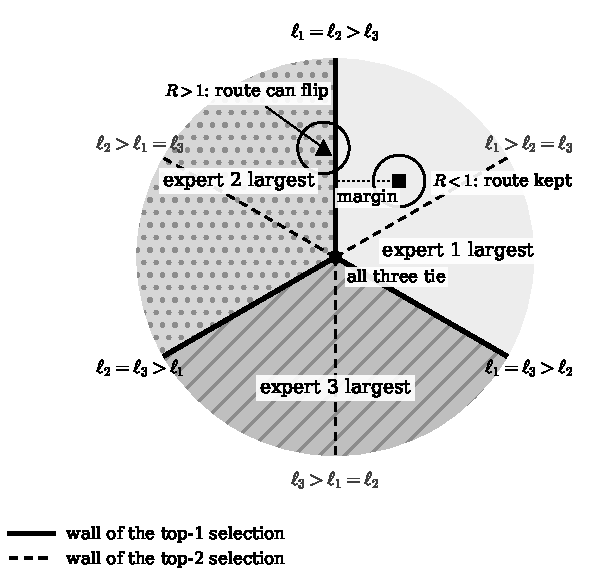
\includegraphics[width=0.62\linewidth]{fig_strata.pdf}
\caption{A selection does not change until a wall is crossed. Three logits are drawn in the plane
orthogonal to the common-mode direction, which no selection depends on. The three lines of ties
meet where all three logits tie, and the faces of the arrangement are that point, six rays and
six sectors. Solid rays are the walls of the top-1 selection and dashed rays the walls of the
top-2 selection. The margin of a logit vector is its distance to the nearest wall, up to a
factor of $\sqrt2$. The same perturbation, drawn as a circle, leaves the selection of the square
point unchanged and can change that of the triangle.}
\label{fig:strata}
\end{figure}

Figure~\ref{fig:strata} shows the arrangement for three logits. The picture gives a law that can
be checked. Add independent Gaussian noise of scale $\sigma$ to
each logit. The difference of two noises has scale $\sqrt2\,\sigma$, so a token with margin $m$
swaps the pair at its boundary with probability $\Phi(-m/(\sqrt2\,\sigma))$, where $\Phi$ is the
standard normal distribution function. If the margins have density $p$ near zero, then to first
order, counting only the nearest wall,
\begin{equation}
\Pr[\text{the selected set changes}] \approx p(0)\int_0^\infty \Phi\!\left(\frac{-m}{\sqrt2\,\sigma}\right)dm
= \frac{p(0)\,\sigma}{\sqrt\pi}.
\label{eq:tube}
\end{equation}
Flips grow linearly with the noise scale, at a rate set by how many tokens sit next to a wall.
Section~\ref{sec:route} compares this with the measured noise sweep.

The other two operators are not strata. The softmax is smooth, and its invariance to a row
constant is a symmetry of constant rank, a quotient. The recurrence has a metric that grows
without bound toward $a = 1$, which is a boundary but not a wall that is crossed. We do not claim
a stratification of the space of consumers.

This section is a definition and a way of organizing four measurements. It is not a theorem, and
two limits should be plain. The quadratic form holds for small perturbations of smooth operators, and
the 3-bit failures below are not small. And it treats one operator at a time. In a model the
output of one operator is the input of the next, so the metric that matters at a weight is the
pullback through everything downstream, which is what the KL at the model's output measures and
what we do not decompose. We do not give a rule for composing operators.

\paragraph{What would count against the claim.} Stated loosely, the claim that sensitivity
follows the consuming operator cannot fail, since \eqref{eq:cost} is defined at the output. It
has content only as a prediction about cheaper proxies. We commit to two. First, a statistic of
the weights alone will misorder tensors that feed different operators, even when their weight
errors are equal. Section~\ref{sec:proj} and the factorial test this, and it holds. Second, at a
matched budget, a rule derived from the consumer will protect better than a rule that ignores it.
Section~\ref{sec:proj:below4} tests this with the rotary wavelength of the key rows. It holds
against random rows, and it fails against a weight statistic: within the rows of one projection,
which all feed the same operator, the relative weight error of a row selects better than the
wavelength does. So the evidence supports the claim across operators and does not support it
within one. Inside a single operator a finer weight statistic can be the better proxy for the
cost \eqref{eq:cost}.

\section{Decision-level agreement and a reference perturbation}\label{sec:agree}

Let $f$ be the base model and $g$ a quantized model, evaluated on $N$ items with labels $y_i$.
We count regressions and recoveries,
\begin{equation}
r = \frac{1}{N}\sum_i \mathbf{1}[f(x_i)=y_i,\ g(x_i)\neq y_i], \qquad
c = \frac{1}{N}\sum_i \mathbf{1}[f(x_i)\neq y_i,\ g(x_i)=y_i],
\end{equation}
whose sum $r+c$ is the flip count of \citet{dutta2024accuracy}, and whose difference $r-c$ is
the accuracy change. Correctness Agreement \citep{rababah2026illusion} equals the base
accuracy minus $r$, so it falls with every regression and cannot see recoveries. The
prediction-level agreement $A = \frac{1}{N}\sum_i \mathbf{1}[f(x_i)=g(x_i)]$ asks whether the
two models give the same answer, right or wrong, and its complement $D = 1-A$ corresponds to
the AllFlips rate of \citet{dutta2024accuracy}.

We also measure a reference-perturbation disagreement $D_0$, the disagreement between two
8-bit requantizations of $f$ that differ only by a seeded dither of a fraction of a quantization
step. $D_0$ measures sensitivity to that procedure and grows with the dither amplitude, as
reported below. It is not an amount of disagreement that the items carry regardless of
quantization, and we do not subtract it as one. We report $D - D_0$ only as a descriptive
comparison, with $D_0$ taken at an amplitude of 0.02 of a step.

\paragraph{Setup.} The task is next-token prediction on the WikiText-2 test split
\citep{merity2017pointer}, in sequences of 256 tokens. An item is one position, and it is
correct when the top-1 token equals the true next token. Every linear layer inside the
transformer blocks is fake-quantized with a symmetric absmax quantizer per output channel, and
the embeddings and language-model head are left in full precision. We run
Qwen2.5-1.5B-Instruct \citep{qwen2025qwen25} on 6{,}120 positions, Mistral-7B-v0.1
\citep{jiang2023mistral} on 12{,}240 and Llama-3.2-3B \citep{grattafiori2024llama3} on
8{,}160. Positions within a sequence are dependent, so these counts overstate the effective
sample size. Every interval in this section is a 95\% bootstrap interval over 2{,}000 resamples
of whole sequences, 24, 48 and 32 of them for the three models. $D - D_0$ is resampled in pairs,
with the same sequences for both terms.

\begin{table}[t]
\centering
\footnotesize
\setlength{\tabcolsep}{4pt}
\begin{tabular}{llrlrrll}
\toprule
model & bits & accuracy & $\Delta$acc & $r$ & $c$ & changed, $1-A$ & $D - D_0$ \\
\midrule
Qwen2.5-1.5B & base & 0.462 & & & & & \\
 & 8 & 0.462 & 0.000 [$-$0.002, 0.001] & 0.003 & 0.004 & 0.022 [0.018, 0.026] & 0.008 [0.004, 0.012] \\
 & 4 & 0.367 & 0.095 [0.085, 0.106] & 0.131 & 0.036 & 0.409 [0.388, 0.429] & 0.395 [0.376, 0.413] \\
 & 3 & 0.002 & 0.459 [0.439, 0.481] & 0.460 & 0.001 & 0.996 [0.995, 0.998] & 0.982 [0.979, 0.985] \\
\midrule
Mistral-7B & base & 0.537 & & & & & \\
 & 8 & 0.538 & 0.000 [$-$0.001, 0.000] & 0.002 & 0.002 & 0.012 [0.010, 0.013] & 0.005 [0.003, 0.007] \\
 & 4 & 0.495 & 0.043 [0.037, 0.048] & 0.072 & 0.029 & 0.232 [0.224, 0.240] & 0.226 [0.217, 0.234] \\
 & 3 & 0.000 & 0.537 [0.519, 0.556] & 0.537 & 0.000 & 0.996 [0.996, 0.996] & 0.990 [0.988, 0.991] \\
\midrule
Llama-3.2-3B & base & 0.496 & & & & & \\
 & 8 & 0.496 & 0.000 [$-$0.002, 0.002] & 0.003 & 0.003 & 0.022 [0.019, 0.025] & 0.010 [0.008, 0.013] \\
 & 4 & 0.429 & 0.067 [0.057, 0.078] & 0.100 & 0.033 & 0.319 [0.305, 0.332] & 0.307 [0.293, 0.320] \\
 & 3 & 0.054 & 0.442 [0.420, 0.463] & 0.451 & 0.009 & 0.919 [0.910, 0.927] & 0.907 [0.899, 0.915] \\
\bottomrule
\end{tabular}
\caption{Accuracy understates how many predictions a quantized model changes. At 4 bits the
fraction of changed predictions, $1-A$, is several times the accuracy drop on all three models,
and the intervals do not overlap. Brackets are 95\% intervals from resampling whole sequences.
$\Delta$acc is base accuracy minus quantized accuracy.}
\label{tab:agree}
\end{table}

\paragraph{Results.} Table~\ref{tab:agree} reports the measure. On Qwen2.5-1.5B at 4 bits,
accuracy falls 9.5 points while 40.9\% of predictions change. On Mistral-7B a 4.3-point
accuracy drop comes with a change in 23.2\% of predictions. At 8 bits on Llama-3.2-3B,
accuracy is unchanged at 0.496, regressions and recoveries are each 0.33\%, and Correctness
Agreement still falls to 0.493, by exactly the regressions. At 8 bits 2.2\% of predictions
change, with an interval of 1.9\% to 2.5\%.

\paragraph{The reference depends on its amplitude.} We repeated $D_0$ over three independent
seed pairs at each of three dither amplitudes. On Llama-3.2-3B it is 1.1\% to 1.3\% at 0.02 of a
step, 1.8\% to 2.0\% at 0.05 and 2.3\% to 2.6\% at 0.1. On Qwen2.5-1.5B the three ranges are 1.1\%
to 1.4\%, 1.8\% to 2.1\% and 2.6\% to 3.0\%, and on Mistral-7B 0.6\% to 0.8\%, 0.9\% to 1.0\% and
1.3\% to 1.4\%. Seeds move $D_0$ by a few tenths of a point and the amplitude moves it by a factor
of two. So $D_0$ is a property of the chosen reference, and the 8-bit disagreement of 2.2\% on
Llama is inside the range that a dither of a tenth of a step produces. We read these numbers
descriptively. Whether near-threshold items explain the 8-bit changes would need their
prediction margins measured, which we have not done.

\section{Projection sensitivity at matched bits}\label{sec:proj}

\citet{rababah2026illusion} report that the query and key projections are more sensitive to
quantization than the value and output projections. In its second version (August 2026) the
paper keeps that claim and measures it on Llama-3.2-3B, Vicuna-7B, Mistral-7B and Llama-3.1-8B,
with moments of the weight entries and with divergences between base and quantized weights,
under llama.cpp legacy schemes and K-quant schemes. It reports that the legacy schemes leave
the per-projection statistics almost unchanged and that the distortions in query and key appear
under the 3-bit and 2-bit K-quant schemes. Its first version advised giving query and key more
precision and compressing value and output harder, and listed in an appendix that the
\texttt{Q2\_K} scheme quantizes query and key at 2 bits, value at 4 and output at 3. The second
version no longer includes that table or that advice. Unequal bits across projections are one
candidate explanation for the reported ordering, and the reported metric, a statistic of the
weights rather than of the model's output, is another. Section~\ref{sec:proj:factorial} tests
both.

\paragraph{Protocol.} We quantize $W^Q$, $W^K$, $W^V$ and $W^O$ with the same symmetric absmax
quantizer per output channel, at $b \in \{8,4,3,2\}$ bits. Sensitivity is read two ways. The
weight lens is the relative Frobenius error of each projection. The functional lens perturbs
one projection type in every layer, leaves the rest in full precision, and measures the mean
$\KL(p_{\text{base}}\,\Vert\,p_{\text{quant}})$ of the next-token distribution over
positions, with the top-1 flip rate. The models are Qwen2.5-1.5B-Instruct, Gemma-3-4B-it
\citep{gemma2025gemma3}, Mistral-7B-v0.1 and Llama-3.2-3B, on 24, 16, 32 and 32 WikiText-2
sequences of 256 tokens. The experiment's script records the hypothesis it was written to
confirm, that query and key would move the output more. The result went the other way.

\begin{table}[t]
\centering
\small
\begin{tabular}{lcrrrr}
\toprule
 & relative Frobenius error & \multicolumn{4}{c}{functional $\KL$, ratio QK / VO} \\
\cmidrule(lr){3-6}
model & QK / VO, all $b$ & 8-bit & 4-bit & 3-bit & 2-bit \\
\midrule
Qwen2.5-1.5B & 0.94--1.00 & 0.38 & 0.26 & 0.17 & 0.27 \\
Gemma-3-4B & 1.03--1.04 & 0.83 & 0.43 & 0.43 & -- \\
Mistral-7B & 1.01--1.13 & 0.29 & 0.29 & 0.44 & 1.05 \\
Llama-3.2-3B & 1.00--1.05 & 0.40 & 0.36 & 2.77 & 1.13 \\
\bottomrule
\end{tabular}
\caption{At matched bits the relative Frobenius errors of the four projections are similar,
while value and output move the output distribution more. A ratio below 1 means query and key
move the output less than value and output. Each ratio is the mean over Q and K divided by the
mean over V and O. Gemma was not run at 2 bits. Single runs, without intervals.}
\label{tab:proj}
\end{table}

\paragraph{Relative Frobenius errors are similar.} Table~\ref{tab:proj} gives the ratio of the
mean relative Frobenius error over query and key to the mean over value and output. It lies
between 0.94 and 1.13 at every bit width on all four models.

\paragraph{The functional ordering is different.} At 8 and 4 bits the functional ratio is below
1 on every model. At 4 bits, perturbing value and output moves the output distribution 3.78
times more than perturbing query and key on Qwen2.5-1.5B, 2.35 times on Gemma-3-4B, 3.41 times
on Mistral-7B and 2.75 times on Llama-3.2-3B. The top-1 flip rates at 4 bits agree. On every
model both value and output flip more tokens than both query and key, for instance 0.075 and
0.048 against 0.034 and 0.036 on Mistral-7B. Under this protocol, compressing value and output
harder than query and key would raise the change in the model's output, not lower it. At 2 bits,
where 68\% to 100\% of top-1 tokens flip under a single projection type, the ratio is near 1 on
Mistral and Llama and stays at 0.27 on Qwen.

\subsection{Where the two orderings part}\label{sec:proj:factorial}

Table~\ref{tab:proj} does not show why the reported ordering differs. Three things differ
between the two protocols: the bit allocation, the quantization scheme and the sensitivity
metric. We crossed them on Llama-3.2-3B and Mistral-7B at two llama.cpp levels, \texttt{Q2\_K}
and \texttt{Q3\_K\_M}. Each level has four arms. The first is the preset as shipped, with its
mixture of tensor types. The second applies one K-quant type to every tensor, which
\texttt{llama-quantize} offers as \texttt{--pure}. The third and fourth use our per-output-channel
absmax quantizer, with each projection at the bit width of its tensor type in the shipped preset,
or with every projection at the level's bit width. In each arm we perturb one projection type in
every layer and read both the weight statistics of the original study's kind and the functional
KL of Section~\ref{sec:proj}. The K-quant weights are dequantized from GGUF files, and the
conversion's row permutation is inverted and checked against a 16-bit GGUF that reproduces the
original weights exactly.

The shipped presets do not give the projections equal bits. In the llama.cpp build we used,
\texttt{Q2\_K} puts query and key at the 2-bit type and output at the 3-bit type on both models.
It puts value at the 4-bit type on Mistral-7B and at the 3-bit type on Llama-3.2-3B, because
that choice depends on the model's ratio of attention heads to key-value heads. \texttt{Q3\_K\_M}
puts query and key at the 3-bit type and value and output at 4-bit and 5-bit types. So the split
attributed above to the first version of \citet{rababah2026illusion} holds for Mistral-7B and
not for Llama-3.2-3B.

\begin{table}[t]
\centering
\small
\begin{tabular}{lllrrr}
\toprule
 & & & \multicolumn{2}{c}{weight statistics, QK / VO} & functional $\KL$ \\
\cmidrule(lr){4-5}
model & level & arm & rel.\ Frobenius & $|\Delta$kurtosis$|$ & QK / VO \\
\midrule
Llama-3.2-3B & \texttt{Q2\_K} & K-quant, shipped mix & 1.97 & 4.24 & 0.91 \\
 & & K-quant, equal type & 1.00 & 1.23 & 0.17 \\
 & & per-channel, shipped bits & 2.27 & 333 & 31.6 \\
 & & per-channel, equal bits & 1.00 & 1.25 & 1.13 \\
 & \texttt{Q3\_K\_M} & K-quant, shipped mix & 2.17 & 1.94 & 1.12 \\
 & & K-quant, equal type & 1.01 & 1.20 & 0.23 \\
 & & per-channel, shipped bits & 2.42 & 3.62 & 15.3 \\
 & & per-channel, equal bits & 1.04 & 1.52 & 2.77 \\
\midrule
Mistral-7B & \texttt{Q2\_K} & K-quant, shipped mix & 2.72 & 6.25 & 1.18 \\
 & & K-quant, equal type & 1.02 & 1.92 & 0.057 \\
 & & per-channel, shipped bits & 3.13 & 205 & 67.3 \\
 & & per-channel, equal bits & 1.01 & 1.47 & 1.05 \\
 & \texttt{Q3\_K\_M} & K-quant, shipped mix & 2.16 & 2.94 & 0.61 \\
 & & K-quant, equal type & 1.01 & 1.02 & 0.17 \\
 & & per-channel, shipped bits & 2.54 & 4.08 & 2.47 \\
 & & per-channel, equal bits & 1.09 & 1.57 & 0.45 \\
\bottomrule
\end{tabular}
\caption{The weight-statistic ordering follows the bit allocation. Each entry is the mean over
query and key divided by the mean over value and output, so a value above 1 says query and key
are the more distorted or the more damaging. With the shipped allocation the weight statistics
put query and key first under both schemes. With equal bits they tie. The functional ratio is
far below 1 under K-quant at equal type. Single runs on 32 sequences, without intervals.}
\label{tab:factorial}
\end{table}

Table~\ref{tab:factorial} gives the outcome, and three things follow from it.

First, the bit allocation moves the weight statistics. Under the shipped mix the relative
Frobenius error of query and key is 2.0 to 2.7 times that of value and output, and the change in
kurtosis is 1.9 to 6.3 times larger. With one type for every tensor the Frobenius ratio is 1.00
to 1.02 and the kurtosis ratio is 1.0 to 1.9. The same holds under our quantizer: 2.3 to 3.1 with
the shipped bits and 1.00 to 1.09 with equal bits. A ranking by these statistics under the
shipped presets therefore ranks the projections by how few bits they were given.

Second, at equal bits under K-quant the metric decides the ordering. The weight statistics tie,
and the functional ratio is 0.17 and 0.23 on Llama and 0.057 and 0.17 on Mistral. Perturbing
value and output moves the output 4 to 17 times more than perturbing query and key. This agrees
with Table~\ref{tab:proj} at 8 and 4 bits, under a different quantization scheme.

Third, the shipped allocation roughly evens out the functional damage. With the presets' extra
bits for value and output, the functional ratio is between 0.61 and 1.18. On this evidence the
presets' choice to spend more bits on value and output is the right way round, and it is the
opposite of the advice to compress them harder.

The scheme matters as well, at low bit widths. Per-output-channel absmax at 2 bits gives a KL
between 2.4 and 5.5 for every projection on both models, where the 2-bit K-quant type gives 0.006
to 0.23, so the per-channel arms at \texttt{Q2\_K} mostly measure collapse. At 3 bits with equal
bits the per-channel ratio is 2.77 on Llama and 0.45 on Mistral, the instability of
Section~\ref{sec:proj:below4}. One weight statistic, a divergence between weight histograms, was
numerically unstable in one arm and we do not report it. The factorial has two models, two
levels and single runs, and we did not run the multiple-choice tasks of the original study. What
it supports is narrow. Under the shipped presets, the weight-statistic ordering is explained by
bit allocation, and it does not carry over to equal bits or to an output-level metric.

\paragraph{Why value and output, a partial test.} A perturbation $\Delta W_K$ of the key weights
changes the score of query position $t$ for source position $s$ by an amount proportional to
$q_t^\top \Delta W_K h_s$, before the rotary embedding. Because $h_s$ varies with the source
token, this error varies across the row of scores, and the softmax cancels only a constant
added to the whole row. Value and output write into the residual stream almost linearly, and
their error reaches the output without passing through a softmax. One hypothesis for the
ordering is that the score errors are partly constant along each row, or small next to the gaps
between scores, so that the softmax suppresses a share of them.

We measured both parts on the four models, perturbing one layer at a time on its own unperturbed
inputs, over 8 sequences. For each query row we split the score error into its row mean and the
centered remainder. At 4 bits the row-constant part carries about half of the squared score
error under a query perturbation, with a median over layers of 0.47 to 0.52 on the four models,
and a quarter to a third under a key perturbation, 0.22 to 0.33. The centered part is small next
to the scores' own spread. Its root mean square is 6\% to 11\% of the within-row deviation of the
scores at 4 bits and 15\% to 24\% at 3 bits, and the attention weights move by a total variation
of 0.02 to 0.06 at 4 bits and 0.06 to 0.13 at 3 bits. So the softmax does cancel a real share of
the query error and a smaller share of the key error, and what remains is small at 4 bits. This
supports the hypothesis without establishing it. The measurement is local to one layer, it has
no interval, and we have not related the centered error to the KL at the model's output across
projections, which is the comparison that would test the account. Gemma-3-4B ran in a different
floating-point format from the other three models, on its text model only.

\subsection{Below 4 bits there is no stable ordering}\label{sec:proj:below4}

At 3 bits two models depart from any ordering. On Llama-3.2-3B the key projection alone gives a
KL of 0.741, against 0.089, 0.125 and 0.174 for query, value and output, while its relative
weight error stays ordinary. Its output movement per unit of relative weight error is 1.71, where
the other projections sit between 0.22 and 0.43. On Qwen2.5-1.5B the output projection rises to
0.624 against 0.183 for value. The fragile projection below 4 bits depends on the model, and the
projection-level weight statistics do not single it out.

For the Llama case the analysis record states a prediction made before the probe ran. Damage
from 3-bit quantization of rows of $W^K$ should rise with the rotary wavelength of the row, and
the profile should be comparatively flat on Mistral-7B, which shows no anomaly. SpQR's
observation that low-frequency rotary weights are the sensitive ones points the same way
\citep{dettmers2024spqr}. The probe groups the rows of every key projection into eight octiles
of rotary wavelength, taken from the model's own frequency buffer, and either quantizes only one
octile or quantizes all rows except one octile.

\begin{table}[t]
\centering
\small
\begin{tabular}{lrr}
\toprule
 & Llama-3.2-3B & Mistral-7B (control) \\
\midrule
KL with all key rows at 3 bits & 0.741 & 0.030 \\
sum of the eight single-octile KLs & 0.173 & 0.031 \\
Spearman correlation of single-octile KL with wavelength & 0.905 & 0.571 \\
two longest octiles, share of the summed single-octile KL & 72\% & 79\% \\
KL removed by sparing the longest octile (12.5\% of rows) & 87\% & 49\% \\
wavelengths of the longest octile (tokens) & $2.0$--$8.2\times10^{7}$ & $2.0$--$5.4\times10^{4}$ \\
Spearman correlation of row weight error with wavelength & 0.12 & 0.22 \\
\bottomrule
\end{tabular}
\caption{The 3-bit key failure on Llama-3.2-3B lives in the long-wavelength rotary rows. The
coupling of damage to wavelength appears on both models, and its size differs by a factor of 25.
Shares are of the summed single-octile KL, which on Llama is far below the joint KL because the
damage is superadditive. The spared share is of the joint KL. Row weight error is nearly
uncorrelated with wavelength, which is a statement about the two orderings of rows and not about
which rows to protect (Table~\ref{tab:protect}).}
\label{tab:wave}
\end{table}

Table~\ref{tab:wave} gives the outcome. The prediction was half right. Damage rises with
wavelength on Llama, with a rank correlation of 0.905 across octiles, and sparing the
longest-wavelength eighth of the rows removes 87\% of the joint KL. The control is not flat.
Mistral's much smaller damage also concentrates in its longest-wavelength rows. The coupling is
common to both models, and what differs is its amplitude, a KL of 0.741 against 0.030. Llama-3.2
stretches its rotary frequencies for long context, and its longest wavelengths reach
$8.2\times10^{7}$ tokens against $5.4\times10^{4}$ for Mistral. The rows that carry those
wavelengths are nearly constant over any practical window. Per-row weight error correlates with
wavelength at 0.12 on Llama and at 0.22 on the control, which suffers 25 times less. The damage is
superadditive. The single-octile KLs on Llama sum to 0.173, against 0.741 when all rows are
quantized together, so the spared-octile numbers are the ones that matter for deployment.

\paragraph{A targeted protection.} Keeping the longest-wavelength eighth of $W^K$ rows in full
precision was then validated through a separate implementation on different hardware. The K-only
3-bit KL on Llama-3.2-3B fell from 0.7352 to 0.0994, a recovery of 86.5\% against the 87\% the
probe predicted. Keeping those rows at 8 bits instead gives the same 0.0994. With one eighth of
the rows at 8 bits and the rest at 3, the key weights average 3.625 bits before scale metadata.
At whole-model 4 bits the protection buys only 2.5\%, from 0.4787 to 0.4668, which fits the
4-bit result above, where value and output dominate.

\paragraph{Are these the right rows?} That result shows that protecting these rows is enough. To
ask whether they are the right rows at that budget, we held the budget at 3.625 bits and changed
only which eighth of the rows of every key projection stays at 8 bits. The conditions are the
longest-wavelength octile, the shortest-wavelength octile, a uniform random eighth of the rows
over five seeds, a random set of rotary frequencies with the structure of an octile over five
seeds, the eighth of rows with the largest relative 3-bit weight error, and the eighth with the
largest output error on calibration activations from 16 training sequences. Evaluation is on 64
sequences of the WikiText-2 validation split, which neither the probe nor the calibration saw.

\begin{table}[t]
\centering
\small
\begin{tabular}{lrrrr}
\toprule
 & \multicolumn{2}{c}{Llama-3.2-3B} & \multicolumn{2}{c}{Mistral-7B} \\
\cmidrule(lr){2-3}\cmidrule(lr){4-5}
eighth of key rows kept at 8 bits & $\KL$ & removed & $\KL$ & removed \\
\midrule
none (all rows at 3 bits) & 0.781 [0.715, 0.837] & & 0.0279 [0.0263, 0.0297] & \\
shortest wavelength & 0.749 [0.688, 0.812] & 4\% & 0.0262 [0.0248, 0.0277] & 6\% \\
random rows, 5 seeds & 0.491 to 0.732 & 6\% to 37\% & 0.0237 to 0.0248 & 11\% to 15\% \\
random frequencies, 5 seeds & 0.350 to 0.627 & 20\% to 55\% & 0.0238 to 0.0251 & 10\% to 15\% \\
longest wavelength & 0.089 [0.083, 0.095] & 89\% & 0.0137 [0.0128, 0.0147] & 51\% \\
largest activation error & 0.031 [0.030, 0.033] & 96\% & 0.0095 [0.0090, 0.0101] & 66\% \\
largest weight error & 0.028 [0.027, 0.029] & 96\% & 0.0073 [0.0069, 0.0078] & 74\% \\
\bottomrule
\end{tabular}
\caption{At a matched budget of 3.625 bits per key weight, the long-wavelength rows are far better
to protect than random rows, and rows chosen by weight error are better still. Held-out
validation text, 64 sequences. Brackets are 95\% intervals from resampling whole sequences. For
the random conditions the range is over seeds.}
\label{tab:protect}
\end{table}

Table~\ref{tab:protect} gives the result. Wavelength is a real criterion. On Llama-3.2-3B the
longest-wavelength eighth removes 89\% of the KL, where a random eighth of rows removes 6\% to
37\% and the shortest-wavelength eighth removes 4\%. The paired interval for the difference in
KL between each random seed and the longest octile lies above 0.22 in every case. The earlier
numbers hold up on held-out text: on the probe's own set this run gives 0.741 and 0.099, against
0.781 and 0.089 on the validation split.

Wavelength is not the best criterion. Protecting the eighth of rows with the largest relative
weight error brings the KL to 0.028, a 96\% reduction, and the paired interval for its difference
from the longest octile is $[-0.066, -0.056]$. The activation-error criterion gives 0.031. The
order is the same on Mistral-7B, where the unprotected damage is 28 times smaller: weight error
removes 74\%, activation error 66\%, the longest octile 51\%, random eighths 10\% to 15\%. The two
criteria do not pick the same rows. On Llama only 23\% of the weight-error rows lie in the longest
octile, and on Mistral 43\%.

This corrects an earlier reading of ours. Table~\ref{tab:wave} shows that row weight error and
wavelength are nearly uncorrelated, and we had taken that to mean that weight statistics do not
locate the damaging rows. At the level of whole projections that still holds, since the four
projections have similar weight error and very different effects. At the level of rows it does
not. A weight-only statistic, the relative quantization error of each row, selects a better eighth
than wavelength does, and it needs no calibration data. The wavelength result stands as a
description of where much of the damage lies and as a structured rule that recovers most of it.
We have not tested combinations of the two criteria, other budgets, or other bit widths.

\section{Inferring the consuming operator}\label{sec:trace}

The results so far name the consumer by hand. Someone knew that keys feed the softmax and that
value and output write the residual stream. The tracer removes that step. Given a model, it maps
every parameter tensor to the operator its output flows into, and from that regime and the
quantization target to a quantization rule.

\begin{table}[t]
\centering
\small
\begin{tabular}{p{2.4cm}p{3.0cm}p{4.3cm}p{4.3cm}}
\toprule
regime & consuming operator & rule for weights & rule for cached activations \\
\midrule
score path & $\mathrm{softmax}(QK^\top)$ & symmetric, lower sensitivity at 4 bits; below 4 bits keep the rows with the largest weight error precise (m, Section~\ref{sec:proj}) & per channel with a zero-point (e) \\
linear residual & writes the residual stream & symmetric, higher sensitivity at 4 bits (m, Section~\ref{sec:proj}) & per vector (e) \\
gated selection & top-$k$ router & keep precise unless the error spread is below the margin (m, Section~\ref{sec:route}) & per channel (d) \\
state decay & linear recurrence & log basis (m, Section~\ref{sec:decay}) & per channel (d) \\
normalization & layer or RMS norm & full precision (d) & full precision (d) \\
unknown & no evidence & per channel with a zero-point (d) & per channel with a zero-point (d) \\
\bottomrule
\end{tabular}
\caption{The rule depends on both the consuming operator and the quantization target. Only the
entries marked (m) are results of this paper. Entries marked (e) were measured in the earlier
cache study. Entries marked (d) are the tracer's defaults. We have not tested them, they are not
recommendations, and the table should not be read as complete. Below 4 bits the weight rules for the score path
and residual are not stable (Section~\ref{sec:proj:below4}).}
\label{tab:regimes}
\end{table}

Table~\ref{tab:regimes} lists the regimes and their rules. Four cells of it are measured here,
the weight rules for the score path, the residual, the router and the decay. The rest is the
tracer's default behavior, listed so that a reader can see what it would do. Two front ends assign the regime. A
structural pass reads each module's type and name. A layer-norm module is a normalization whatever
its name. A router gate is selection, and the pass excludes the gate projection of a SwiGLU
feed-forward block, which is not a router. A second pass traces the graph with torch.fx
\citep{reed2022torchfx}, finds the sink operators, softmax, top-$k$ and cumulative scan, and
follows each back to the linear layers that feed it. That pass labels the score, gate and state
tensors even when their names give nothing away. Where the graph pass has positive evidence it
overrides the structural guess. Where a model cannot be traced, the structural result stands. An
unclassified tensor gets the conservative default, which keeps scale on a coordinate whose
consumer is unknown.

\paragraph{Measurement.} The paper's own results do not depend on the tracer. Every consumer in
Sections~\ref{sec:proj} to~\ref{sec:decay} was named by hand. We measured the tracer on two groups
of models whose consuming operators are known by construction. The first group is eight library
architectures, Llama, Mistral, Qwen2, Gemma, GPT-2, Mixtral, OLMoE and Mamba, each built from its
configuration at a small size with random weights, since only the module graph and the parameter
names matter. The second group is four small modules written for the test, an attention block, a
top-$k$ router, a diagonal recurrence and a SwiGLU block, each in two namings: the usual names,
and names that carry no signal. A tensor is scored only if its consumer is declared. Biases,
embeddings and convolutions are not scored.

\begin{table}[t]
\centering
\small
\begin{tabular}{lrrr}
\toprule
 & tensors scored & correct & graph trace succeeds \\
\midrule
eight library architectures, both passes & 200 & 200 & 0 of 8 \\
four small modules, usual names, both passes & 13 & 12 & 4 of 4 \\
four small modules, uninformative names, both passes & 13 & 12 & 4 of 4 \\
four small modules, uninformative names, names only & 13 & 9 & \\
\bottomrule
\end{tabular}
\caption{The graph pass works where it can trace and never engages on the library
architectures. On those the tracer falls back to names in every case, and the 200 correct labels
show only that its name rules cover the eight naming schemes, because the ground truth there is
itself read from names. With uninformative names the graph pass recovers the query, key, gate and
decay tensors that the name pass misses.}
\label{tab:tracer}
\end{table}

Table~\ref{tab:tracer} gives the result, and it limits what can be claimed. Symbolic tracing with
torch.fx failed on all eight library architectures, each time on an input check in the model's
forward pass. So on every real architecture we tried, the tracer is the name pass alone. Its 200
labels there are all correct, including the two hard cases at scale: the Mixtral and OLMoE gates
are labelled as routers, and the gate projection of every SwiGLU block is not. That is evidence
that the name rules fit these eight architectures. It is not evidence of inference from the
graph, since the ground truth is read from the same names.

The graph pass is tested by the second group. With uninformative names the name pass gets 9 of 13
tensors right: it cannot see the query, key, gate or decay tensors and labels them by its
default. With the graph pass added the score is 12 of 13. The one error is a false positive of
the graph pass. In the recurrence, the linear map that feeds the scan is labelled as state decay,
because the backward walk from the scan tags every linear layer on the way. The same module with
the usual names exposes a second defect, in the name pass: a parameter named \texttt{in\_proj} is
labelled as a score path, a rule written for a fused attention projection. GPT-2's fused
projection, which holds query, key and value in one tensor, is labelled as a score path as well,
which is right for two thirds of it. The tracer also reports a successful trace only when it
finds a softmax, a top-$k$ or a scan, so its own flag cannot tell a failed trace from a graph
with none of them.

The tracer is therefore a set of name rules that fit current architectures, plus a graph pass
that works on modules simple enough to trace. Using it on a production model needs a tracer that
handles the library's forward passes, and a calibration batch to confirm each regime.

\section{Routing flips concentrate on small margins}\label{sec:route}

A top-$k$ router selects experts by the order of its logits $\ell = W_g x$. Adding the same
constant to every logit leaves the selection unchanged, so the common-mode part of a
quantization error is free. Let the margin $m$ of a token be the gap between its $k$-th and
$(k{+}1)$-th largest logits.

\paragraph{A sufficient condition.} If a perturbation $\delta$ satisfies
$|\delta_i - \bar\delta| < m/2$ for every expert $i$ and some constant $\bar\delta$, the top-$k$
set does not change. For a selected expert $i$ and an unselected expert $j$ we have
$\ell_i - \ell_j \geq m$, and a swap needs $\delta_j - \delta_i > \ell_i - \ell_j$, which the
bound rules out. The same argument gives a form that is easy to measure. Let
\begin{equation}
R = \frac{\max_i \delta_i - \min_i \delta_i}{m}
\end{equation}
be the spread of the error over the experts divided by the margin. If $R < 1$ the top-$k$ set
does not change. $R$ does not change when the router's weights are multiplied by a positive
constant.

\paragraph{Setup.} We capture the router logits of Mixtral-8x7B-Instruct-v0.1
\citep{jiang2024mixtral}, 8 experts with top-2 routing over 32 layers, and of OLMoE-1B-7B-0924
\citep{muennighoff2025olmoe}, 64 experts with top-8 routing over 16 layers, on WikiText-2. That
gives 131{,}072 and 262{,}144 routing decisions. We then quantize the gate weights at 4
and 3 bits with one uniform grid per tensor from its smallest to its largest entry, recompute the
routing, and split tokens at the median margin. For the same tokens we compute $R$ from the
router's input and the weight error. The logits are recomputed from the router's captured input
and its stored weights, and the flip rates so obtained reproduce those of the routing run. Separately, we add
independent Gaussian noise to each logit at a scale $\sigma$ set relative to the median margin.

\begin{table}[t]
\centering
\small
\begin{tabular}{lrr}
\toprule
 & Mixtral-8x7B (top-2) & OLMoE-1B-7B (top-8) \\
\midrule
margin at the top-$k$ boundary, median (10th percentile) & 0.485 (0.076) & 0.0015 (0.0002) \\
gate weights at 4 bits, top-$k$ set flips (low / high margin) & 16.6\% (10.7) & 91.8\% (1.09) \\
gate weights at 3 bits, top-$k$ set flips (low / high margin) & 34.0\% (2.69) & 98.7\% (1.01) \\
gate weights at 4 bits, $R$: 10th percentile, median, 90th & 0.40, 1.28, 8.2 & 7.5, 27.9, 191 \\
gate weights at 4 bits, tokens with $R < 1$ & 40.9\% & 0.003\% \\
gate weights at 3 bits, $R$: 10th percentile, median, 90th & 0.90, 2.9, 18.5 & 12.1, 48.4, 345 \\
gate weights at 3 bits, tokens with $R < 1$ & 12.5\% & 0\% \\
logit noise $\sigma = 0.25\,m_{50}$, flips (low / high margin) & 9.2\% (2007) & 10.6\% (1740) \\
logit noise $\sigma = 0.5\,m_{50}$ & 17.9\% (16.7) & 20.2\% (22.6) \\
logit noise $\sigma = m_{50}$ & 34.1\% (3.4) & 35.7\% (4.6) \\
logit noise $\sigma = 2\,m_{50}$ & 58.3\% (1.6) & 57.7\% (2.1) \\
\bottomrule
\end{tabular}
\caption{Flips concentrate on low-margin tokens on both routers. The figure in parentheses is the
flip rate of tokens below the median margin divided by that of tokens above it. Under 4-bit gate
quantization the concentration survives on Mixtral, while on OLMoE nearly every token's expert set
changes. The ratio $R$ of error spread to margin separates the two. Absolute margins are not
comparable across the two models (see text). Single runs.}
\label{tab:route}
\end{table}

\paragraph{Results.} Table~\ref{tab:route} reports both routers. Under logit noise at a quarter of
the median margin, low-margin tokens flip 2{,}007 times more often than high-margin ones on Mixtral
and 1{,}740 times more often on OLMoE, and the ratio falls toward 1 as the noise grows past the
margins. Under gate quantization the two routers part. At 4 bits, Mixtral's top-2 set changes for
16.6\% of tokens, with low-margin tokens flipping 10.7 times more often, while OLMoE's top-8 set
changes for 91.8\% of tokens with almost no concentration.

The difference in absolute margins, a median of 0.485 against 0.0015, does not explain this by
itself. Multiplying a router's weights by a positive constant multiplies every margin by it, and
under a per-tensor uniform grid it multiplies the quantization error by the same constant, so
every routing decision and every flip stays the same. The scale-free quantity is $R$.

$R$ separates the two routers. On Mixtral at 4 bits its median is 1.28, and 40.9\% of tokens have
$R < 1$. None of those tokens changes its route in any of the 32 layers, as the condition
requires, and the 16.6\% of flips all come from the remaining tokens. By layer, the share of
tokens with $R < 1$ runs from 27\% to 73\%. On OLMoE at 4 bits the median of $R$ is 27.9, its
10th percentile is 7.5, and 0.003\% of tokens have $R < 1$. The error spread exceeds the margin
by an order of magnitude for nearly every token, which is why 91.8\% of expert sets change and
why the margin no longer predicts which ones. At 3 bits the share with $R < 1$ falls to 12.5\% on
Mixtral and to zero on OLMoE.

\paragraph{The linear law.} Equation~\eqref{eq:tube} predicts the flip rate under logit noise
from the density of margins near zero. We estimate that density from the 10th percentile of the
margin, $p(0) \approx 0.1/m_{10}$, which assumes the density is flat below it. At
$\sigma = 0.25\,m_{50}$ the prediction is 9.0\% for Mixtral's top-2 boundary and 10.5\% for
OLMoE's top-8 boundary, against measured flip rates of 9.2\% and 10.6\%. For the top-1 boundary
of the same two routers it is 8.2\% and 9.7\% against 8.4\% and 9.6\%. Doubling the noise to
$0.5\,m_{50}$ multiplies the measured rate by 1.95 and 1.90 at the top-$k$ boundary and by 2.00
and 1.89 at the top-1 boundary, close to the factor of 2 that a linear law gives, and the growth
slows at larger noise as the nearest wall stops being the only one in reach. The agreement is
better than the approximation deserves, since at this noise scale $\sigma$ already exceeds
$m_{10}$. We take it as support for the picture and not as a calibrated formula.

The practical rule is then conditional. A router can be quantized where the error spread stays
below the margin for most tokens, and $R$ can be computed from the gate weights and a sample of
router inputs before any routing is recomputed. Mixtral's gate at 4 bits is a borderline case, and
OLMoE's gate at 4 or 3 bits under this quantizer is not usable. The condition is sufficient and
not necessary: on Mixtral most tokens with $R \geq 1$ also keep their route. We tested one
quantizer, a single grid per tensor, and a per-expert grid may give a different $R$.

\section{State decay is set by its basis}\label{sec:decay}

A per-channel linear recurrence $h_t = a\,h_{t-1} + b_t$ has steady-state gain $1/(1-a)$, whose
derivative in $a$ is $1/(1-a)^2$. An error in the decay of a slow channel, with $a$ near 1, is
amplified far more than the same error in a fast channel, and it accumulates over the sequence. A
quantizer for the decay should therefore spend its levels near $a = 1$. Mamba \citep{gu2024mamba}
stores the continuous decay as $A = -\exp(A_{\log})$ and discretizes it as $a = \exp(\Delta A)$.
Then $\log(-\log a) = \log\Delta + A_{\log}$, so a uniform grid on $A_{\log}$ is a uniform grid on
the logarithm of the decay rate $-\log a$, whose inverse is the time constant, and it places fine
levels where $a$ is near 1.

\paragraph{Setup.} On Mamba-790m, with 48 layers and 2{,}359{,}296 decay channels, we
fake-quantize each layer's decay tensor at 3 bits in one of two bases. The linear grid has 8
uniformly spaced levels from the tensor's smallest to its largest value of $A$. The log grid has 8
uniformly spaced levels from the smallest to the largest value of $A_{\log}$. In exact arithmetic every
level of the linear grid is negative, so no channel is mapped to $A = 0$, where its decay would
vanish. In 32-bit arithmetic that does not hold for the top level, as reported below.
We put the result back into the model and measure WikiText-2 perplexity over up to 40 windows of
2{,}048 tokens, in 32-bit floating point so that a collapsed model reports a finite value.

\paragraph{Results.} The baseline perplexity is 11.65. The log grid gives 14.44. The linear grid
on $A$ collapses the model, with a perplexity above $10^{9}$. Two implementations of the same
grid, on the same windows, give $1.0\times10^{10}$ and $5.9\times10^{9}$. They differ in whether
the grid's endpoints and step are held in 64-bit or 32-bit floating point. The top level is
computed as an offset of order $10^{6}$ plus a multiple of the step, which cancels to a value
near zero, so its sign is decided by rounding. It lands at or above zero, where the harness clamps
the decay rate to a small positive floor, in 6 of the 48 layers in one implementation and in 8
in the other. The perplexity of the collapsed model depends on those bits, and neither figure is
a stable number. The
largest steady-state gain among the model's decays is 42{,}690.

\paragraph{What the linear grid does.} We counted, for every channel, the ratio of its quantized
decay rate to its original one. The decay rates within a tensor span many orders of magnitude,
from $2\times10^{-5}$ to $2.9\times10^{6}$ over the model with a median of 9.6. The step of the
linear grid is 383 times the median decay rate of a typical layer, and at least 38 times in every
layer. So 99.8\% of all channels, and at least 99.0\% in every layer, round to the grid's top
level, the one nearest zero. In most layers that level is negative and their decay
becomes far slower, and in the layers named above it is clamped to the floor. Over the model 94\% of channels slow by more than a factor of 10, and the median channel by
a factor of about 200. Under the log grid the median rate ratio is 0.99, no channel slows by a
factor of 10, and 28\% change by more than a factor of 2 in either direction.

The collapse is therefore a statement about what this grid does to the decay rates, as we had
suspected. To see whether it is an artifact of one grid, we added a second linear grid that
resolves each row of the decay tensor over its own range. That grid still puts 43.5\% of channels
on its top level and slows 9\% of them by more than a factor of 10, and its perplexity is
$4.1\times10^{6}$. It is three orders of magnitude better than the per-tensor linear grid and
still a collapse. Two linear grids fail and the log grid does not.

\paragraph{A second model.} We repeated the three grids on Mamba-370m, a second checkpoint of
the same architecture with 48 layers and 1{,}572{,}864 decay channels. Its baseline perplexity is
13.99. The log grid gives 18.94. The per-tensor linear grid again puts 99.8\% of channels on its
top level, slows 96\% of them by more than a factor of 10, and collapses the model, with a
perplexity above $10^{11}$. The per-row linear grid puts 51\% of channels on its top level and
gives $5.1\times10^{7}$. Under the log grid no channel slows by a factor of 10 and 35\% change by
more than a factor of 2. The pattern is the same on both models. The log grid costs more here
than on the larger model, a factor of 1.35 in perplexity against 1.24. Both models are from one
family and one training recipe, so this is a replication within the Mamba architecture and not a
test on a different state-space model. We have not tested a linear grid built to preserve each
slow channel's rate.

\section{Limitations}\label{sec:limits}

The paper offers one definition and four case studies. It has no single sensitivity that covers
all four operators beyond the definition of Section~\ref{sec:pullback}, and no rule for composing
operators. Every experiment uses fake quantization, quantizing and dequantizing weights or
activations and running in floating point. Intervals are given for the agreement measure and the row-protection
controls, by resampling whole sequences. The matched-bit ratios of Table~\ref{tab:proj}, the
factorial, the score-error decomposition, the routing study and the decay study are single runs
without intervals. The task is next-token prediction on WikiText-2, and we did not run the
multiple-choice tasks of \citet{rababah2026illusion}. The factorial covers two models and two
llama.cpp levels, and its conclusion is about the shipped presets, not about every scheme. The
softmax account of the ordering is supported by a local measurement and not tested at the
model's output. Below 4 bits we claim only instability. The wavelength mechanism rests on one
model and one control at one bit width, and its prediction was recorded in an analysis note
rather than a sealed registration. The row-protection controls use one budget and one bit width,
and the weight-error criterion that wins them was a control, not a method we set out to propose.
The tracer's graph pass failed to trace every library architecture we tried, so on those it is a set of name rules, scored against ground truth that is itself read from names. The routing study uses one quantizer, a
single grid per tensor, on two routers. The decay study uses two checkpoints of one architecture.

\section*{Broader impact statement}

Quantization lets models run on smaller hardware at lower energy. Reading sensitivity at the
model's output makes silent behavior change easier to detect before deployment. We see no direct
negative impact beyond those of the models being compressed.

\section*{Use of large language models}

Large language model assistants were used to write and run analysis code, to organize results and
to draft this manuscript. The authors reviewed and edited the text and checked each reported
number against the recorded results.

\section*{Reproducibility}

The anonymized supplement contains the code for every experiment and the JSON record of each run.
A notebook rebuilds every number in Tables~\ref{tab:agree} to~\ref{tab:route} and in
Section~\ref{sec:decay} from those records and compares it with the value printed in the paper.
It does not rerun the models. The scripts that produced the records are included, and they need a
GPU. A Lean 4 file, checked against Mathlib with no proof left open, verifies the identities the
text relies on: the relations among the agreement counts, the cancellation of a row constant by
the softmax, the split of a score error into row-constant and centered parts, the sufficient
conditions for a top-$k$ set to survive, the invariance of routing to a common scale, the two
inclusions of subspaces to which Whitney's conditions reduce for the arrangement of ties, and the
identities of the decay parameterization. It makes no statement about any trained model.

\bibliography{references}
\bibliographystyle{tmlr}

\end{document}
